\noindent Pro ideální OTA zesilovač (vstupní i výstupní impedance nulové) je možno odpor nahradit obvodem s uzemněným neinvertujícím vstupem a zpětnou vazbou z invertujícího vstupu na výstup a to hodnotou
\begin{align}
R_{in} = \frac{1}{g_{m}},
\end{align}
kde $g_{m}$ označuje transkonduktanci zesilovače. Prohození invertujícího a neinvertujícího vstupu vede na opačnou polaritu.
\begin{figure}[H]
\centering
\includegraphics[scale=0.7]{image10.png}
\caption{Náhradní obvod pro uzemněný rezistor \cite{12}}
\end{figure}
\noindent Pro nahrazení indukčnosti o impedanci $Z_L = 1/(sC)$ lze použít obvod s třemi OTA. Uzemněny jsou invertující vstup prvního OTA a neinvertující druhého. Použita je zpětná vazba z výstupu na neinvertující vstup prvního OTA. Propojení výstupu prvního OTA na invertující vstup druhého OTA je realizován přes uzemněný kapacitor. \\
Vyjádřením napětí a proudů v obvodu bylo získáno napětí na kapacitoru a vstupní proud
\begin{align}\label{s:vzt2}
V_C &= \frac{g_{m1}}{sC}V_1 \\
I_1 &= g_{m2}V_C = \frac{g_{m1}g_{m2}}{sC}V_1.
\end{align}
Výsledná indukčnost - impedance vstupu byla vyjádřena vztahem \ref{s:vzt2}.
\begin{align}
Z_{in}(s) = \frac{V_1}{I_1} = s\frac{C}{g_{m1}g_{m2}}
\end{align}
\noindent Byl obdržen induktor o hodnotě
\begin{align}
L = \frac{C}{g_{m1}g_{m2}}.
\end{align}
\begin{figure}[H]
\centering
\includegraphics[scale=0.55]{image13.png}
\caption{Náhradní obvod pro indukčnost \cite{12} \label{s:IND}}
\end{figure}
\noindent Pro uzemněnou indukčnosti o impedanci $Z_L = 1/(sC)$ byl použit obvod na Obrázku \ref{s:IND}. Vyjádřením napětí a proudů v obvodu bylo získáno napětí na kapacitoru a vstupní proud
\begin{align}
V_C &= \frac{g_{m1}}{sC}V_1 \\
I_1 &= g_{m2}V_C = \frac{g_{m1}g_{m2}}{sC}V_1.
\end{align}
Výsledná indukčnost - impedance vstupu byla vyjádřena vztahem
\begin{align}
Z_{in}(s) = \frac{V_1}{I_1} = s\frac{C}{g_{m1}g_{m2}}.
\end{align}
\begin{figure}[H]
\centering
\includegraphics[scale=1]{image12.png}
\caption{Náhradní obvod pro neuzemněnou indukčnost pro $g_{m1} = g_{m2}$\cite{12}}
\end{figure}
\subsection{Odvození DP 2. řádu}\label{s:ODV}
\noindent Náhradní obvod, ze kterého bude spočítána přenosová funkce pro přenos filtru druhého řádu, popisuje Obrázek \ref{s:DPO}.
\begin{figure}[H]
\centering
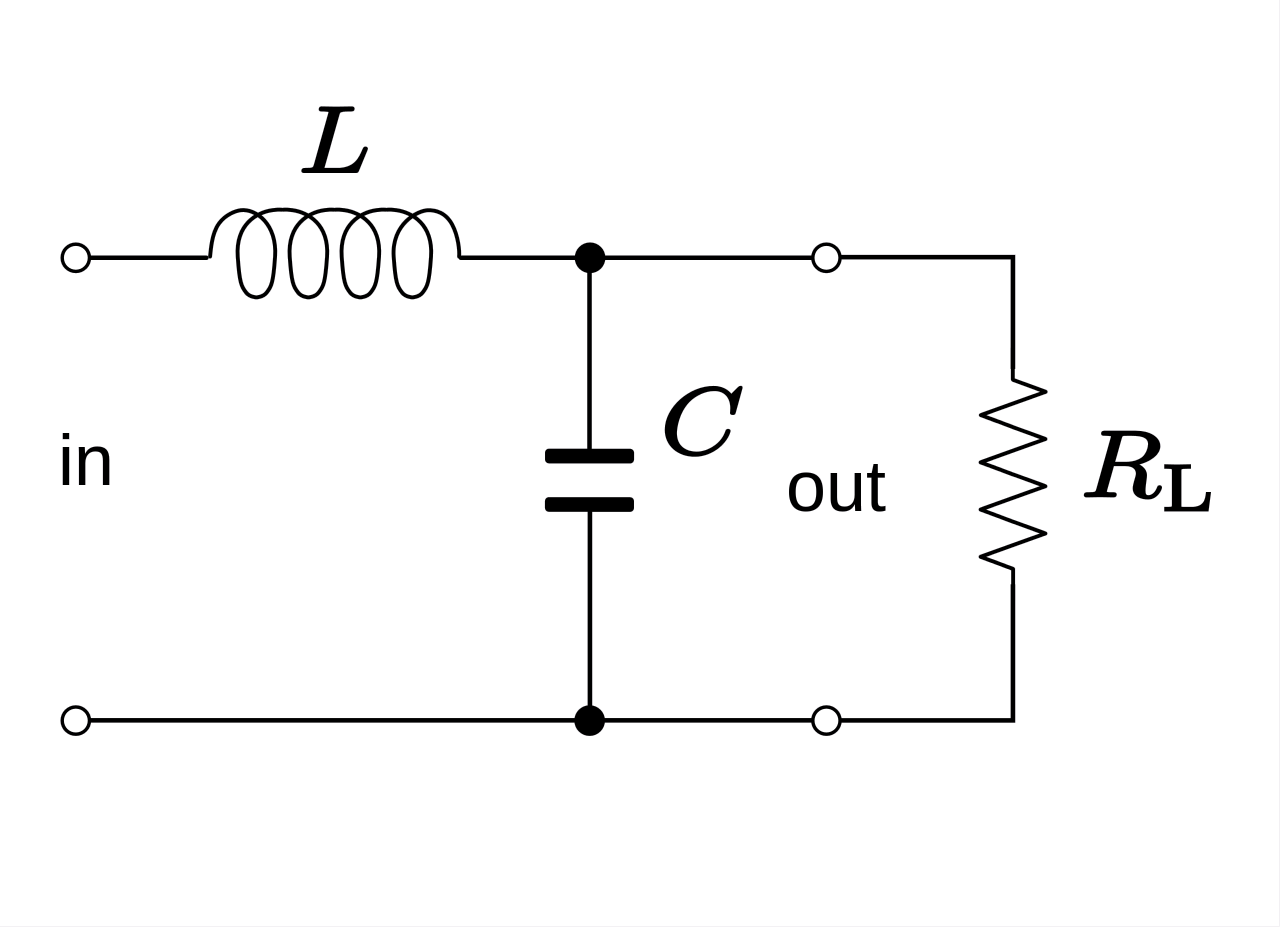
\includegraphics[scale=0.15]{RLC_low-pass.png}
\caption{Dolní propust 2. řádu \cite{11} \label{s:DPO}}
\end{figure}
\noindent Přenos obvodu byl vyjádřen jako
\begin{align}
H(s) = \frac{U_{out}}{U_{in}} = \frac{Z_2}{Z_1}, \quad Z_1 = sL,\quad Z_2 = \frac{\frac{R}{sC}}{R + \frac{1}{sC}}.
\end{align}
Výsledný přenos je roven 
\begin{align}
H(s) = \frac{\frac{\frac{R}{sC}}{R + \frac{1}{sC}}}{sL + \frac{\frac{R}{sC}}{R + \frac{1}{sC}}}.
\end{align}
Elementárními algebraickými úpravami a následným vynásobením členem $1/(LRC)$ byl získán výsledný přenos.
\begin{align}\label{s:vzt4}
H(s) = \frac{R}{s^2LRC + sL + R} = \frac{\frac{1}{LC}}{s^2 + \frac{s}{RC} + \frac{1}{LC}}.
\end{align}
\noindent Využitím poznatků ze Sekce \ref{s:NAH} je možno za odpor a indukčnost dosadit do vztahu \ref{s:vzt4}. Byly uvažovány kapacitory o stejné hodnotě C.
\begin{align}
H(s) = \frac{\frac{1}{\frac{C^2}{g_{m1}g_{m2}}}}{s^2 + \frac{s}{\frac{C}{g_{m2}}} + \frac{1}{\frac{C^2}{g_{m1}g_{m2}}}} = \frac{\frac{g_{m1}g_{m2}}{C^2}}{s^2 + \frac{sg_{m2}}{C} + \frac{g_{m1}g_{m2}}{C^2}} = \frac{g_{m1}g_{m2}}{s^2C^2 + sg_{m2}C + g_{m1}g_{m2}}.
\end{align}
Porovnáním jmenovatele se jmenovatelem přenosu filtru 2. řádu byl obdržen vztah
\begin{align}
s^2 + s\frac{\omega _c}{Q} + \omega _c^2 &= s^2C^2 + sg_{m2}C + g_{m1}g_{m2}\\
s^2 + s\frac{\omega _c}{Q} + \omega _c^2 &= s^2 + \frac{sg_{m2}}{C} + \frac{g_{m1}g_{m2}}{C^2}.
\end{align}
Z tohoto vztahu byl vyjádřen mezní kmitočet jako 
\begin{align}
\omega _c^2 &= \frac{g_{m1}g_{m2}}{C^2} \\
\omega _c &= \sqrt{\frac{g_{m1}g_{m2}}{C^2}}
\end{align}
a činitel jakosti dosazením za $\omega _c$
\begin{align}
Q = \frac{\omega _c}{\frac{g_{m2}}{C}} = \sqrt{\frac{g_{m1}}{g_{m2}}}.
\end{align}
Pokud navíc byly uvažovány stejné transkonduktance $g_{m1}, \ g_{m2} = g_m$, byl obdržen výsledek
\begin{align}
\omega _c &= \sqrt{\frac{g_m^2}{C^2}},\\
Q &= \sqrt{1} = 1.
\end{align}